\documentclass[11pt]{article}
\usepackage[review]{acl}
\usepackage{times}
\usepackage{latexsym}
\usepackage[T1]{fontenc}
\usepackage[utf8]{inputenc}
\usepackage{microtype}
\usepackage{inconsolata}
\usepackage{graphicx}
\usepackage{booktabs}
\usepackage{multirow}
\usepackage{longtable}
\usepackage{amsmath}
\usepackage{amssymb}
\usepackage{url}

\providecommand{\tightlist}{%
  \setlength{\itemsep}{0pt}\setlength{\parskip}{0pt}}

\title{From Prompting to Structured Alignment: Individual, Population, and Temporal Boundaries of LLM Survey Simulation}
\author{Anonymous ACL submission}

\begin{document}
\maketitle

\begin{abstract}
Large language models are increasingly used as virtual survey respondents, but
most evaluations treat surveys as one-shot prompting tasks. We present a
data-centric pipeline that reconstructs voter--candidate interactions from
ANES, aligns a compact 8B model with survey distributions via LoRA, and
evaluates both individual-level prediction and population-level simulation. On
unseen respondents in the same era, the fine-tuned model reaches an MAE of
20.84, a correlation of 0.679, and a choice accuracy of 0.518 against a chance
level of 0.163; a gradient-boosted baseline on the same features reaches 20.58,
0.714, and 0.534, and paired bootstrap shows no significant MAE or choice
difference. On GSS policy attitudes, fine-tuning reduces marginal and joint
Jensen--Shannon divergence by 91\% and 86\% on the EDC configuration. We then
show a sharp temporal boundary: across the 2019--2024 waves, individual-level
correlation decays from 0.722 to near zero, and both the LLM and the tabular
baseline collapse in 2024. Structured alignment is necessary but not sufficient
for social simulation, and temporal distribution shift should be treated as a
first-class evaluation axis.
\end{abstract}

\section{Introduction}\label{introduction}

Questionnaire surveys are the backbone of empirical social science and policy evaluation, but they are expensive, slow, and increasingly difficult to field at scale. Large language models (LLMs) have been proposed as virtual survey respondents: given a demographic profile and a question, a model can produce an answer without recruiting a single participant \citep{argyle2022, dillion2023, kim2023}. The promise is attractive, but most existing work evaluates the model as a one-shot prompt. A profile is placed in the context window, a question is asked, and the answer is scored. This setup measures how well a model can role-play a respondent in a single turn; it does not test whether the model has internalized the structure of survey responses, whether its outputs are coherent at the population level, or whether the behavior survives a change in the political environment.

We take a different view. Survey responses are generated by a structured process: a voter's partisan identity, ideological position, and demographics interact with a candidate's attributes, and the resulting evaluations follow regularities that are stable within an era and can shift across eras. If an LLM is to act as a credible respondent, it should be trained on that structure rather than prompted with it. We therefore build a data-centric pipeline that reconstructs voter--candidate and voter--group interactions from the American National Election Studies (ANES), aligns a compact 8B model with the resulting distribution via LoRA, and evaluates the model at both the individual and the population level. We then use the same pipeline to study when this alignment stops working.

Our first contribution is a reproducible data construction and audit. The raw ANES feature table contains two defects that are easy to miss and that materially change results: duplicate thermometer items stored under trailing-period names (\texttt{obama.} and \texttt{obama}), and social-group thermometers stored in the same column as candidate thermometers. We quantify both, separate the targets, and reduce 132,948 raw rows to 98,159 clean interaction-level rows. We also show that ANES is a panel: 3,080 of 3,165 respondents appear in more than one wave, and there are no test-only respondents in 2022/2024. A temporal split therefore measures transfer to a later wave, not generalization to unseen individuals. We report both a temporal protocol and a respondent-disjoint protocol, and we make the distinction explicit throughout.

Our second contribution is an individual-level evaluation that is deliberately conservative. On unseen respondents in the 2016--2019 waves, the fine-tuned model reaches an MAE of 20.84, a correlation of 0.679, and a rating-induced choice accuracy of 0.518 against a chance level of 0.163. A gradient-boosted model on the same features reaches 20.58, 0.714, and 0.534. Paired bootstrap shows that the MAE and choice differences are not significant, while the correlation difference is: the tabular baseline is at least as good as the LLM. We report this result rather than hiding it. The value of the LLM is not that it is a better point predictor; it is that the same model can produce a distribution over the rating scale and can be extended to population-level generation.

Our third contribution is a population-level evaluation. On the GSS policy-attitude data, fine-tuning on a reconstructed joint distribution reduces marginal and joint Jensen--Shannon divergence by 91\% and 86\% on the EDC configuration, and by up to 76\% and 64\% on EHC. The gains are not explained by retrieval augmentation or by quota sampling; supervised fine-tuning is the driver. The EDC result is strong, the EHC result is moderate, and we report both.

Our fourth contribution is a temporal boundary analysis. Across the 2016--2024 waves, individual-level correlation falls from 0.722 in 2019 to 0.478 in 2020, 0.408 in 2022, and -0.056 in 2024. The tabular baseline decays later but collapses in the same way (0.746, 0.560, 0.657, -0.008). Adding the 2022 wave to training does not help. The failure is in the survey distribution, not in the language model alone. We argue that temporal shift should be treated as a first-class evaluation axis for LLM survey simulation, alongside individual accuracy and distributional alignment.

The remainder of the paper is organized as follows. Section 2 reviews related work. Section 3 describes the data construction, cleaning, features, sampling, and evaluation protocols. Section 4 presents the method: prompting, LoRA fine-tuning, two rating readouts, baselines, and the FAS pipeline. Section 5 reports the individual-level results, Section 6 the population-level results, and Section 7 the temporal analysis. Section 8 reports ablations and subgroup analyses. Section 9 discusses limitations and ethical considerations, and Section 10 concludes.

\section{Related Work}\label{related-work}

\subsection{LLMs as virtual survey respondents}\label{llms-as-virtual-survey-respondents}

A growing line of work uses LLMs to simulate survey responses. \citet{argyle2022} condition language models on demographic backstories and show that the resulting ``silicon samples'' can approximate subgroup opinions; \citet{santurkar2023} show that the same models are skewed toward WEIRD populations; \citet{dillion2023} ask whether models can replace human participants; and \citet{kim2023} use models to augment surveys. Later work extends the paradigm to random silicon sampling \citep{sun2024}, cross-survey probing \citep{zhou2024}, and the construction of multi-domain benchmarks \citep{zhao2025}. \citet{cao2025} specialize models to survey response distributions for global populations.

Most of this work evaluates a model as a one-shot respondent: a profile and a question are placed in the prompt, and the answer is compared with a survey margin. The model is not trained on the survey structure, and the evaluation rarely separates individual-level accuracy from population-level distributional alignment. Our work builds on the benchmark of \citet{zhao2025} but turns it into a training and evaluation pipeline: we reconstruct interaction-level data, fine-tune a compact model, and report individual, population, and temporal results separately.

\subsection{Persona, role-play, and personalization}\label{persona-role-play-and-personalization}

A related literature studies how well models maintain a persona. \citet{park2024} simulate 1,000 people with generative agents; \citet{wang2024} evaluate personality fidelity in role-playing; \citet{xu2024} ask whether models can make persona-driven decisions; \citet{salemi2024} incorporate user profiles into dialogue; and \citet{ng2024} measure how well models ``echo'' a user. This work is primarily about behavioral consistency within a conversation. Our setting is different: the model is not asked to stay in character over a dialogue but to reproduce the statistical structure of survey responses across a population. Persona fidelity and distributional fidelity are complementary, and our data-design choices (candidate metadata, interaction features) can be read as a way to make the persona operational.

\subsection{Fine-tuning for social simulation}\label{fine-tuning-for-social-simulation}

Fine-tuning has been used to align models with political or social preferences \citep{chu2023, zhao2023}, often with the goal of mimicking a group's voice. Our goal is not preference alignment but competence alignment: we want the model to learn the rules that map a voter profile and a candidate to a rating, not to adopt a particular ideology. This distinction matters for evaluation. A model that has learned the rules should generalize to unseen respondents and candidates; a model that has learned a group's voice may reproduce the margin without the mechanism. The respondent-disjoint protocol in Section 3.6 is designed to test the former.

\subsection{Population-level distribution alignment}\label{population-level-distribution-alignment}

Synthetic population generation has a long history outside LLMs. Iterative proportional fitting \citep{deming1940, fienberg1970} reconstructs a joint distribution from marginal and lower-order constraints, and LOESS \citep{cleveland1979} provides a flexible univariate smoother. We combine these classical tools with a language model: the joint distribution is reconstructed with an ensemble of extrapolators and IPF, and the model is fine-tuned on samples from the reconstructed joint. The resulting system can generate a population rather than a point prediction, which is the capability that distinguishes FAS from PAS.

\subsection{Temporal generalization and distribution shift}\label{temporal-generalization-and-distribution-shift}

Survey attitudes change across waves, and a model trained on historical data may not transfer to a future election. Prior work on LLM survey simulation has generally evaluated on a single wave or on a pooled sample, which can hide temporal decay. Our temporal analysis is, to our knowledge, the first to report a monotonic per-year decay of individual-level correlation for both a fine-tuned LLM and a feature-engineered baseline on the same ANES panel. The result is a caution for the use of LLM simulations in forecasting settings and a motivation for treating temporal shift as a separate evaluation axis.

\subsection{Positioning}\label{positioning}

Our work sits at the intersection of the three lines above. Unlike prompting-only silicon sampling, we train on interaction-level data. Unlike preference alignment, we target distributional and individual-level fidelity. Unlike prior FAS work, we add a panel-aware evaluation protocol and a temporal boundary analysis. The negative results are part of the contribution: the fine-tuned model is competitive rather than superior at the individual level, and both the LLM and the tabular baseline fail under a four-year shift. We report these findings explicitly so that subsequent work can build on a calibrated picture of what structured alignment does and does not buy.

\section{Data Construction}\label{data-construction}

\subsection{Source surveys}\label{source-surveys}

We build the individual-level corpus from the American National Election Studies (ANES) pilot waves of 2016, 2018, 2019, 2020, 2022, and 2024. The raw respondent-by-target table contains 132,948 rows, 3,165 unique respondents, and 29 candidate targets. For the population-level component we use the General Social Survey (GSS) waves of 2004, 2008, 2012, 2014, 2016, 2018, 2021, and 2022, with 2024 as the target year.

\subsection{Cleaning}\label{cleaning}

The raw ANES feature table contains two defects that materially affect any downstream evaluation. First, several feeling-thermometer items are stored twice with a trailing period (\texttt{obama.} and \texttt{obama}, \texttt{hrc.} and \texttt{hrc}), producing 8,165 duplicate rows. Second, social-group thermometers (\texttt{black}, \texttt{white}, \texttt{dem}, \texttt{rep}) are stored in the same column as candidate thermometers, producing 23,060 rows in which the ``candidate'' is in fact a group. Treating these rows as candidate preferences contaminates both training and evaluation.

We therefore normalize target names by lower-casing and stripping trailing periods, separate candidate targets from group targets, drop rows with missing or out-of-range scores (3,588), and deduplicate on \texttt{(respondent,\ year,\ target)} (8,141 rows). The resulting candidate table contains \textbf{98,159} interaction-level rows. We retain the original row index so that every cleaned row can be traced back to the raw table. Table~\ref{tab:audit} summarizes the audit.

\begin{table}[t]
\centering
\small
\begin{tabular}{lr}
\toprule
Item & Value \\
\midrule
Raw rows & 132,948 \\
Clean rows & 98,159 \\
Respondents & 3,165 \\
Respondents in multiple waves & 3,080 \\
Test-only respondents & 0 \\
\texttt{train\_t} / \texttt{val\_t} / \texttt{test\_t} & 6,516 / 2,501 / 3,421 \\
\texttt{train\_r} / \texttt{test\_r} / \texttt{test\_tr} & 5,094 / 6,014 / 226 \\
\bottomrule
\end{tabular}
\caption{Data audit and split statistics.}
\label{tab:audit}
\end{table}


\subsection{Interaction-level representation}\label{interaction-level-representation}

A wide-format ANES row stores one voter and many thermometer columns, which implicitly treats a rating as a property of the voter and suppresses voter-target interactions. We instead represent each observation as a triple

\[
(v_i,\ c_j,\ y_{ij}\mid t_i),
\]

where \(v_i\) is the voter profile, \(c_j\) the target, \(y_{ij}\in[0,100]\) the feeling thermometer, and \(t_i\) the survey year. This yields one row per voter-target pair and makes the interaction structure explicit.

Candidate identity is decoupled from candidate attributes. Each candidate is represented by a metadata vector

\begin{equation*}
\resizebox{\columnwidth}{!}{$\displaystyle 
\mathcal{M}[c] = (\text{party},\ \text{ideology},\ \text{age},\ \text{position},\ \text{incumbent}),
$}
\end{equation*}

so that the model learns \(P(y\mid v,\mathcal{M}[c],t)\) rather than memorizing a candidate name. The same transformation is applied to social groups: a group is described by its category (race, party, ideology, or social movement), ideological position, and valence. The group corpus contains 61,710 voter-group pairs over nine groups (Black, White, Hispanic, and Asian Americans; the Democratic and Republican parties; Socialists and Capitalists; and Feminists).

\subsection{Social-cognitive features}\label{social-cognitive-features}

On top of the interaction-level rows we compute a compact set of features that encode theoretical primitives of political cognition. Partisan reasoning is captured by

\begin{equation*}
\resizebox{\columnwidth}{!}{$\displaystyle 
\text{party\_match}(v,c)=
\begin{cases}
+1 & \text{if } \text{party}_v=\text{party}_c,\\
-1 & \text{if } v \text{ is an independent},\\
0 & \text{otherwise}.
\end{cases}
$}
\end{equation*}

Spatial reasoning is captured by the seven-point ideological distance

\begin{equation*}
\resizebox{\columnwidth}{!}{$\displaystyle 
\text{ideo\_dist}(v,c)=\lvert \text{lcself}_v-\text{ideology}_c\rvert\in[0,6],
$}
\end{equation*}

and a composite similarity index combines party, ideology, race, gender, and age:

\[
\begin{aligned}
\text{sim}(v,c) ={}& 0.25\,\mathbb{1}[\text{party match}] \\
&+0.25\,\mathbb{1}[\text{same ideological side}] \\
&+0.20\,\mathbb{1}[\text{race match}] \\
&+0.15\,\mathbb{1}[\text{gender match}] \\
&+0.15\left(1-\frac{\lvert \text{age}_v-\text{age}_c\rvert}{100}\right).
\end{aligned}
\]

Finally, cross-pressure indicators flag cases in which partisan and ideological cues conflict:

\[
\begin{aligned}
\text{CP}_1 &= \mathbb{1}[\text{party match}=1 \land \text{ideo\_dist}\ge 3],\\
\text{CP}_2 &= \mathbb{1}[\text{party match}=0 \land \text{ideo\_dist}\le 1],\\
\text{CP}_3 &= \mathbb{1}[\text{sim}\ge 0.7 \land \text{party match}=0].
\end{aligned}
\]

These features are not arbitrary predictors: they operationalize partisan identity, spatial proximity, and ambivalence, and they are the same features we later give to the tabular baseline.

\subsection{Distribution-aware sampling}\label{distribution-aware-sampling}

Uniform sampling from a survey over-represents common profiles and under-represents the tails and conflict cases that carry most of the theoretical interest. We therefore draw the training pool with nine complementary strategies: balanced coverage of the score range, hard cases near the middle of the scale, party-by-ideology cells, similarity-stratified bins, cross-pressure cases, extreme scores, incumbent effects, temporal coverage, and candidate-specific balance. The resulting pool contains 6,516 rows and is intentionally not a uniform sample; the test sets, in contrast, are built from all cleaned rows in the target years so that evaluation is not shaped by the same sampling design.

\subsection{Evaluation protocols and the panel caveat}\label{evaluation-protocols-and-the-panel-caveat}

ANES is a panel: 3,080 of the 3,165 respondents appear in more than one wave, and every respondent observed in 2022 or 2024 also appears in 2016--2020. There are \textbf{zero} test-only respondents. A temporal split can therefore measure transfer to a later wave, but it cannot isolate generalization to unseen individuals.

We report two complementary protocols. The \textbf{temporal protocol (T)} trains on 2016--2020 (6,516 rows), validates on 2022 (2,501), and tests on 2024 (3,421). The \textbf{respondent protocol (R)} splits respondents 80/20 by a hash of the respondent identifier, independent of year: 5,094 training rows and 6,014 test rows. We also report a strict cell, \textbf{T×R}, containing the 226 rows from 2024 whose respondents are in the 20\% held-out set. Within each protocol the splits are disjoint; the two protocols intentionally overlap across each other. R is our main in-distribution test, while T measures the temporal boundary.

For groups, coverage is uneven across waves (three groups in 2016, six in 2018, four in 2019, nine in 2020, two in 2022), so a temporal group split is not meaningful. We instead use a within-2020 block split (80/20 respondents, all nine groups) and a multi-year respondent split over the six groups with reliable identifiers.

\subsection{Population-level survey data}\label{population-level-survey-data}

For the population-level task we reconstruct the joint distribution of three policy attitudes from GSS. We use two configurations: \textbf{EDC} (education, drug addiction, crime) and \textbf{EHC} (environment, health, cities). Each attribute takes three levels (\texttt{too\ little}, \texttt{about\ right}, \texttt{too\ much}). Eight historical waves provide the time series; the target is 2024. Section 4.5 describes how the joint distribution is extrapolated and used to build fine-tuning tasks.

\section{Method}\label{method}

\subsection{Task definitions}\label{task-definitions}

We study two levels of survey simulation.

\textbf{Partial Attribute Simulation (PAS).} Given a voter profile \(v\), a target \(c\) with metadata \(\mathcal{M}[c]\), and a year \(t\), the model predicts a feeling-thermometer score

\[
\hat y = f_\theta(v,\mathcal{M}[c],t)\in[0,100].
\]

For evaluation we also form a discrete choice. For each respondent-year pair we collect the candidates the respondent rated, take the model's highest-scoring candidate

\[
\hat c^* = \arg\max_{c\in\mathcal{C}(v,t)} f_\theta(v,\mathcal{M}[c],t),
\]

and compare it with the candidate with the highest ground-truth rating. We call this \textbf{rating-induced choice}; it avoids requiring a separate vote-choice variable, which is unavailable for all waves.

\textbf{Full Attribute Simulation (FAS).} Given three categorical policy attitudes \((A,B,C)\), the model must generate samples whose marginal and joint distributions match a target population. We evaluate the generated sample against the empirical 2024 distribution.

\subsection{Prompting and LoRA fine-tuning}\label{prompting-and-lora-fine-tuning}

Each PAS example is rendered as a short survey vignette. The system message defines the task and fixes the output format (a single integer in \([0,100]\)). The user message contains the voter profile (age, gender, race, education, party identification, ideology), the candidate block (name, party, position, age), and the interaction block (party alignment, ideological distance, age difference, year). Group examples use the same structure with a group block instead of a candidate block.

We fine-tune a compact instruction-tuned model (Qwen3-8B) with LoRA. For a frozen weight matrix \(W_0\), LoRA learns a low-rank update

\[
W' = W_0 + \frac{\alpha}{r}BA,
\qquad B\in\mathbb{R}^{d\times r},\ A\in\mathbb{R}^{r\times k},
\]

with rank \(r=8\), scaling \(\alpha=32\), dropout \(0.1\), applied to the query, key, value, output, gate, up, and down projections. We train for three epochs with a learning rate of \(10^{-4}\), an effective batch size of 16, and a maximum sequence length of 512. The loss is the causal language-modeling loss on the answer tokens only; prompt tokens are masked with \(-100\). This yields 21.8M trainable parameters, or 0.27\% of the model. We fine-tune three seeds (42, 43, 44) and report mean and standard deviation.

\subsection{Rating readouts and choice}\label{rating-readouts-and-choice}

A fine-tuned model can be read out in two ways.

\textbf{Generation.} We decode greedily for at most eight tokens and parse the first integer in \([0,100]\). This preserves individual variation and is our primary readout for choice.

\textbf{Anchor likelihood.} Because the tokenizer splits most two- and three-digit numbers into several tokens, a single-position softmax over 0--100 is not available. We instead score eleven anchor strings \(a\in\{0,10,\dots,100\}\) by their sequence log-probability under the prompt,

\[
s(a)=\sum_{k=1}^{|a|}\log p_\theta\!\left(a_k \mid \text{prompt}, a_{<k}\right),
\]

normalize with a softmax over the eleven anchors, and report both the expectation (a calibrated scalar) and the argmax (a discrete rating). The anchor readout requires one forward pass per anchor but no generation, and it exposes a full distribution over the rating scale.

For choice we use the same rule in both readouts: within each respondent-year group, the candidate with the highest predicted score is selected. We report the observed accuracy together with the chance accuracy \(1/|\mathcal{C}(v,t)|\), which is 0.5 for the two-candidate 2024 wave.

\subsection{Baselines}\label{baselines}

We compare against three baselines. \textbf{HistGB} and \textbf{Ridge} are trained on the same tabular features used to render the prompts (demographics, party, ideology, candidate metadata, and the interaction features of Section 3.4); they provide a strong non-LLM reference and test whether the language model adds anything beyond feature engineering. The \textbf{base LLM} uses the same prompts without fine-tuning. All baselines are evaluated on the same splits and metrics.

\subsection{Population-level simulation (FAS)}\label{population-level-simulation-fas}

FAS has three stages.

\textbf{Extrapolation.} For every univariate and pairwise cell we observe a short time series and predict the target year with a four-model ensemble,

\[
\hat p(t^*) =
\frac{1.0\,\hat p_{\text{poly}}+1.0\,\hat p_{\text{loess}}+0.6\,\hat p_{\text{exp}}+0.8\,\hat p_{\text{lin}}}{3.4},
\]

where the components are quadratic regression, LOESS with a tri-cube kernel, an exponential trend, and linear regression. Predictions are clipped to \([0,1]\) and renormalized.

\textbf{Joint reconstruction.} The predicted marginals and pairwise tables are combined with iterative proportional fitting (IPF). Starting from the independence approximation \(Q^{(0)}(a,b,c)=P(A)P(B)P(C)\), we alternate multiplicative updates to match each pairwise table and each marginal, run 800 iterations, normalize, and apply Laplace smoothing. The result is a coherent three-way distribution \(Q^*(A,B,C)\).

\textbf{Task construction.} We sample synthetic populations from \(Q^*\) and convert them into five instruction-following task types: batch generation (50\%), prior-constrained sampling (25\%), scenario variation (15\%), subgroup analysis with Wilson confidence intervals (7\%), and iterative correction (3\%). A compact model is fine-tuned on this mixture. At evaluation time we compare generated samples with the empirical 2024 distribution.

\subsection{Metrics and reproducibility}\label{metrics-and-reproducibility}

For PAS we report mean absolute error (MAE), root mean squared error (RMSE), Pearson and Spearman correlation, a relaxed accuracy (same 20-point bin or absolute error \(\le 10\)), rating-induced choice accuracy, and expected calibration error (ECE). For FAS we report Jensen--Shannon (JS) divergence and symmetric KL divergence on each marginal and on each pairwise joint, averaged over the three attributes or three pairs.

All results are produced by scripts under \texttt{experiments/}; predictions are saved per row, and every table in the paper is generated from those files. The main PAS results use three seeds; the ablations and the temporal mitigation use one seed and are reported as such. The code, splits, and prediction files are released with the paper.

\section{PAS Experiments}\label{pas-experiments}

\subsection{Setup}\label{setup}

We fine-tune Qwen3-8B with LoRA on the 6,516-row training pool described in Section 3.5, using three seeds (42, 43, 44). The main in-distribution evaluation uses the respondent protocol (R) restricted to the 2016, 2018, and 2019 waves: 2,726 rows from respondents never seen during training. The 2020 wave is treated as a near-domain set, and 2022/2024 form the temporal test analyzed in Section 7. We report MAE, Pearson correlation, rating-induced choice accuracy, and chance accuracy. Baselines are HistGB and Ridge on the same tabular features, plus the base model with the same prompts but no fine-tuning. All confidence intervals are bootstrap 95\% intervals over rows (MAE, correlation) or respondent-year groups (choice).

\subsection{In-distribution results}\label{in-distribution-results}

Table~\ref{tab:pas} reports the main result. The fine-tuned LLM reaches an MAE of 20.84 {[}20.38, 21.30{]}, a correlation of 0.679 {[}0.666, 0.692{]}, and a choice accuracy of 0.518 {[}0.481, 0.552{]} against a chance level of 0.163. HistGB reaches 20.58 {[}20.01, 21.12{]}, 0.714 {[}0.696, 0.733{]}, and 0.534 {[}0.498, 0.569{]}; Ridge is weaker at 22.47, 0.655, and 0.484.

\begin{table}[t]
\centering
\small
\resizebox{\columnwidth}{!}{%
\begin{tabular}{lccc}
\toprule
Model & MAE [95\% CI] & Correlation [95\% CI] & Choice [95\% CI] \\
\midrule
Fine-tuned LLM (3 seeds) & 20.84 [20.38, 21.30] & 0.679 [0.666, 0.692] & 0.518 [0.481, 0.552] \\
HistGB & 20.58 [20.01, 21.12] & \textbf{0.714} [0.696, 0.733] & 0.534 [0.498, 0.569] \\
Ridge & 22.47 & 0.655 & 0.484 \\
Base LLM & 24.16 [23.44, 24.88] & 0.593 & 0.479 \\
\bottomrule
\end{tabular}}
\caption{PAS in-distribution results on unseen respondents (2016--2019). Chance choice accuracy is 0.163.}
\label{tab:pas}
\end{table}



The honest reading is that the LLM is \textbf{competitive with, but not superior to, a strong tabular baseline}. A paired bootstrap over the same 2,726 rows confirms this: for seed 42 the LLM--GBM difference in MAE is \(+0.60\) \([-0.19, +1.42]\) (seeds 43 and 44: \(+0.02\) and \(+0.19\)), and the difference in choice is \(+0.026\) \([-0.007, +0.062]\); both intervals include zero. The correlation difference is \(-0.039\) \([-0.056, -0.021]\), consistently negative across seeds. Fine-tuning, by contrast, improves MAE by 2.98 \([2.10, 3.82]\) relative to the base model, with a correlation gain of \(+0.082\) and a choice gain of \(+0.081\). We therefore do not claim that the language model is a better individual-level predictor than feature-engineered regression. What the LLM adds is different: a single model that consumes the same survey vignette can produce a full rating distribution (Section 4.3) and can be extended to population-level generation (Section 6), whereas the tabular baselines cannot.

The gap to the prompt-only model is large. On the same in-distribution rows, the base LLM reaches an MAE of 24.16 {[}23.44, 24.88{]}, a correlation of 0.593, and a choice accuracy of 0.479; on the 2020 wave it degrades to an MAE of 44.89 and a correlation of -0.389. Fine-tuning is therefore necessary for the model to behave like a survey respondent rather than a generic assistant (Table~\ref{tab:pas}, last row).

\subsection{Per-year behavior}\label{per-year-behavior}

Table~\ref{tab:year} and Figure~\ref{fig:temporal} break the in-distribution result down by wave. Performance is best in 2019 (MAE 19.20, correlation 0.722, choice 0.663 against chance 0.150) and weaker in 2016 (22.45, 0.588, 0.329 against 0.112). HistGB shows the same ordering, with a higher correlation in all three waves (0.611, 0.729, 0.746) and a similar choice profile (0.256, 0.544, 0.639). The LLM narrows the gap in 2019 but does not overtake the baseline.

\begin{table*}[t]
\centering
\small
\resizebox{\linewidth}{!}{%
\begin{tabular}{lccccccc}
\toprule
& & \multicolumn{3}{c}{Fine-tuned LLM} & \multicolumn{3}{c}{HistGB} \\
\cmidrule(lr){3-5}\cmidrule(lr){6-8}
Year & $n$ & MAE & corr & choice & MAE & corr & choice \\
\midrule
2016 & 697 & 22.45 & 0.588 & 0.329 & 22.32 & 0.611 & 0.256 \\
2018 & 727 & 22.25 & 0.670 & 0.530 & 22.02 & 0.729 & 0.544 \\
2019 & 1,302 & 19.20 & 0.722 & 0.663 & 18.85 & 0.746 & 0.639 \\
2020 & 2,868 & 25.39 & 0.478 & 0.326 & 23.41 & 0.560 & 0.278 \\
2022 & 194 & 27.76 & 0.408 & 0.674 & 27.98 & 0.657 & 0.804 \\
2024 & 226 & 37.30 & $-$0.056 & 0.448 & 35.52 & $-$0.008 & 0.460 \\
\bottomrule
\end{tabular}}
\caption{PAS by survey year on the held-out respondents. The 2022 and 2024 waves have two candidates, so chance choice accuracy is 0.5.}
\label{tab:year}
\end{table*}



This pattern is consistent with the interpretation that both models recover the same partisan and ideological structure; the LLM's advantage, if any, is not in average accuracy but in the form of its output. Figure~\ref{fig:scatter} shows the corresponding density: predictions are correlated with the ground truth but are compressed toward the middle of the scale, with a visible band at 50. The compression is a property of the fine-tuned readout, not of the correlation alone, and it motivates the anchor readout discussed next.
\begin{figure}[t]
\centering
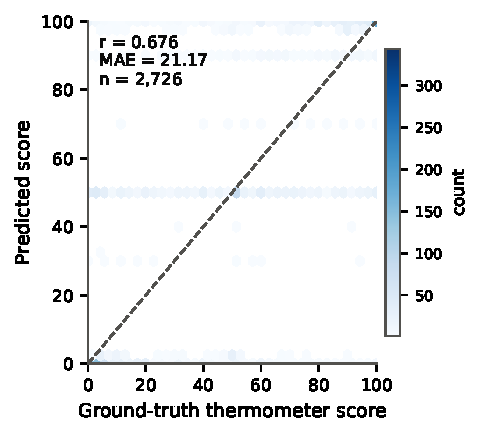
\includegraphics[width=0.9\columnwidth]{figures/fig4_pas_scatter.pdf}
\caption{In-distribution prediction density.}
\label{fig:scatter}
\end{figure}

\subsection{Generation versus anchor readout}\label{generation-versus-anchor-readout}

The two readouts in Section 4.3 behave differently. On the full 2024 test set (seed 42), the anchor readout gives a lower MAE than generation (34.99 versus 35.79) and a much lower ECE (2.90 versus 10.46), while choice accuracy is similar (0.547 versus 0.536). However, the anchor predictions have a standard deviation of only 2.1 and a correlation with the truth of 0.003: the low ECE is produced by an almost constant prediction near 40, not by genuine calibration. Generation has a larger spread (standard deviation 12.3) and a correlation of -0.009 on the same rows. Neither readout recovers individual signal in 2024.

On the in-distribution years, where predictions do vary, generation is the primary readout because it preserves individual differences and yields the choice results above. The anchor readout is useful as a diagnostic of the model's rating distribution, but it should not be reported as evidence of calibration unless the prediction spread is reported alongside it. We return to this point in Section 7, where the 2024 collapse is analyzed as a temporal rather than a readout failure.

\subsection{Discussion}\label{discussion}

Three conclusions follow. First, structured fine-tuning is necessary: the base model is both biased and unstable, and its 2020 correlation is negative. Second, the fine-tuned model is a credible individual-level simulator in-distribution, but it does not beat a feature-engineered GBM; the contribution of the language model must therefore be argued on other grounds. Third, the readout matters: a low ECE can be an artifact of prediction collapse, so calibration claims must be paired with correlation and spread.

The results support a narrow form of C1: structured survey data alignment gives a compact LLM genuine individual-level signal on unseen respondents in the same era. They do not support a claim of LLM superiority over tabular baselines, and we do not make one.

\section{FAS Experiments}\label{fas-experiments}

\subsection{Setup}\label{setup-1}

The population-level evaluation uses the GSS data described in Section 3.7. For each of the two three-attribute configurations (EDC and EHC), we reconstruct the 2024 joint distribution from eight historical waves, sample 400 synthetic respondents, and compare the generated sample with the empirical 2024 sample (1,552 respondents for EHC and 1,601 for EDC). We report Jensen--Shannon (JS) divergence on the three marginals and the three pairwise joints, averaged within each family. Lower is better. Symmetric KL is reported as a secondary metric.

We compare six generation conditions: the base model, direct supervised fine-tuning (SFT), retrieval-augmented generation without fine-tuning (RAG), RAG plus SFT, a second SFT run with a different task mixture (v2), a third SFT run (v3), and a quota-annealing sampler. All generation runs use the same prompts and the same target year; only the training or sampling procedure changes.

\subsection{Main results}\label{main-results}

Table~\ref{tab:fas} and Figure~\ref{fig:fas} summarize the results. On EDC, the base model produces a marginal JS of 0.0552 and a joint JS of 0.1181. Direct SFT reduces these to 0.0048 and 0.0160, a relative reduction of \textbf{91\% and 86\%}. The best SFT run (v3) reaches 0.0040 and 0.0215, i.e., \textbf{93\% and 82\%}. On EHC, the base model starts at 0.0319 and 0.1001; direct SFT reaches 0.0167 and 0.0470 (48\% and 53\%), and v3 reaches 0.0077 and 0.0363 (\textbf{76\% and 64\%}).

The EDC result supports the claim that fine-tuning substantially improves population-level distributional alignment, including the pairwise structure that a marginal-only sampler would miss. The EHC result is weaker: the marginal reduction is large in the best run, but the joint reduction is only about two thirds. We report both configurations rather than selecting the favorable one, and we scope the ``80\% reduction'' claim to EDC.

\begin{table*}[t]
\centering
\small
\resizebox{\linewidth}{!}{%
\begin{tabular}{llcccc}
\toprule
Config & Run & $n$ & Coverage & Marginal JS & Joint JS \\
\midrule
\multirow{6}{*}{EDC} & Base & 400 & 1.000 & 0.0552 & 0.1181 \\
 & SFT & 381 & 0.953 & 0.0048 & 0.0160 \\
 & SFT (v3) & 400 & 1.000 & \textbf{0.0040} & 0.0215 \\
 & RAG & 376 & 0.940 & 0.0473 & 0.1096 \\
 & RAG + SFT & 381 & 0.953 & 0.0054 & 0.0176 \\
 & Quota & 395 & 0.988 & 0.0091 & 0.0216 \\
\midrule
\multirow{6}{*}{EHC} & Base & 351 & 0.877 & 0.0319 & 0.1001 \\
 & SFT & 400 & 1.000 & 0.0167 & 0.0470 \\
 & SFT (v3) & 400 & 1.000 & \textbf{0.0077} & \textbf{0.0363} \\
 & RAG & 379 & 0.948 & 0.0404 & 0.1095 \\
 & RAG + SFT & 380 & 0.950 & 0.0152 & 0.0427 \\
 & Quota & 400 & 1.000 & 0.0175 & 0.0522 \\
\bottomrule
\end{tabular}}
\caption{FAS distributional alignment on GSS (JS divergence, lower is better). Coverage is the fraction of the 400 requested rows returned.}
\label{tab:fas}
\end{table*}


\begin{figure*}[t]
\centering
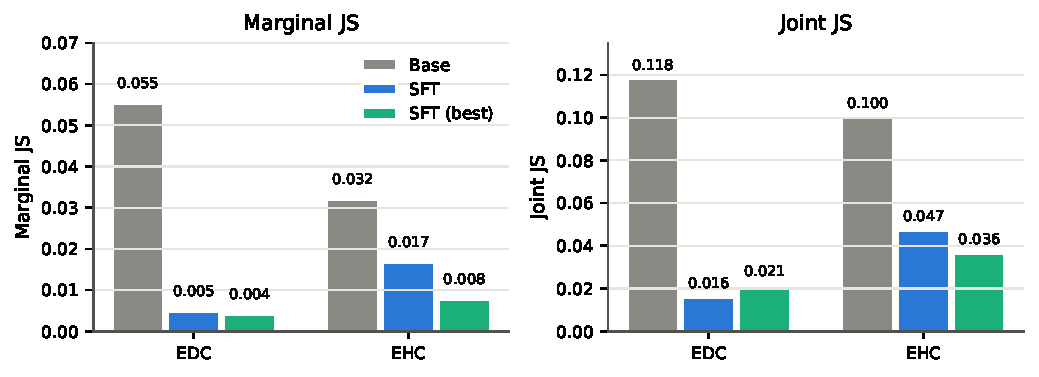
\includegraphics[width=\linewidth]{figures/fig3_fas_js.pdf}
\caption{FAS distributional alignment.}
\label{fig:fas}
\end{figure*}

The two metrics do not always agree. On EHC, the symmetric KL of the joint distribution increases from 0.4289 (base) to 0.5487 (direct SFT) even though JS falls from 0.1001 to 0.0470. KL is sensitive to near-zero cells and to the 400-sample size; JS is bounded and more stable. We therefore treat JS as the primary metric and KL as a diagnostic, and we do not claim a KL improvement for EHC.

\subsection{Component analysis}\label{component-analysis}

Three comparisons isolate the source of the gain.

\textbf{RAG is not the driver.} RAG without fine-tuning is close to the base model on EDC (0.0473 marginal, 0.1096 joint) and slightly worse than the base on EHC (0.0404, 0.1095). Adding retrieval does not by itself teach the model the target distribution.

\textbf{SFT is the driver.} RAG plus SFT performs like direct SFT on both configurations (EDC 0.0054/0.0176; EHC 0.0152/0.0427). The improvement comes from supervised exposure to the reconstructed distribution and the five task types, not from retrieval.

\textbf{Quota annealing is not better.} The quota sampler reaches 0.0091/0.0216 on EDC and 0.0175/0.0522 on EHC, worse than direct SFT on both. We therefore do not use quota annealing in the main method.

\subsection{Why EDC and EHC differ}\label{why-edc-and-ehc-differ}

EDC and EHC are not equally predictable. EDC (education, drugs, crime) has stronger and more stable temporal trends in the GSS waves, so the extrapolated 2024 joint is closer to the truth and the fine-tuning signal is cleaner. EHC (environment, health, cities) is more volatile and less correlated across attributes; the ensemble extrapolation is less accurate, and the joint reconstruction has more room for error. We treat this as an empirical difference between configurations rather than as evidence that the method is uniformly effective.

\subsection{Sample completeness}\label{sample-completeness}

The generation conditions differ in how many valid rows they produce. The base model returns 351 of 400 requested rows on EHC (coverage 0.877), while the SFT runs return 399--400; on EDC, direct SFT returns 381 rows (coverage 0.953) and the v3 run returns 400. Because the distributional metrics are computed on the returned rows, a condition that produces fewer rows is not penalized for the missing mass. To make the comparison conservative, we charge every missing row as maximally wrong (the maximum JS for a categorical distribution is \(\ln 2\)). Under this adjustment, the base model's EHC marginal and joint JS rise from 0.0319/0.1001 to 0.1168/0.1850, while the fully covered v3 run stays at 0.0077/0.0363. On EDC, direct SFT's raw 0.0048/0.0160 becomes 0.0377/0.0489 under the same penalty, whereas v3, which returns all 400 rows, is unaffected at 0.0040/0.0215.

We therefore treat v3 as the cleanest headline result: it achieves full coverage on both configurations and the lowest raw JS. Direct SFT still shows a large improvement, but part of its apparent advantage on EDC is due to the 19 missing rows. We report raw and coverage-adjusted values in Table~\ref{tab:fas} and recommend that future work report both.

\subsection{Discussion}\label{discussion-1}

The FAS results support C2 for EDC: supervised fine-tuning on a reconstructed joint distribution reduces both marginal and joint divergence by roughly an order of magnitude, and the gain is not explained by retrieval or quota sampling. For EHC the gain is real but smaller, and the KL diagnostic moves in the opposite direction for the joint. The honest summary is that the method works well when the underlying temporal trends are stable and the attributes are correlated, and less well when they are not.

This is also the part of the pipeline where the language model contributes something the tabular baseline cannot: it generates a synthetic population rather than a point prediction, and it can be asked to condition, perturb, or correct that population in natural language. The individual-level results in Section 5 are competitive rather than superior; the population-level results are the clearest evidence for the value of the approach.

\section{Temporal Analysis}\label{temporal-analysis}

\subsection{Setup}\label{setup-2}

The temporal protocol (T) trains on 2016--2020 and tests on 2024. We also report a per-year view of the respondent protocol: for each wave from 2016 to 2024, we evaluate the same fine-tuned model on the rows contributed by the 20\% held-out respondents. This holds respondent identity fixed while letting the survey year vary, which isolates the temporal component from respondent memorization. The 2024 wave is additionally evaluated on the full 3,421-row test set (all respondents), and we compare with HistGB trained on the same features.

\subsection{The decay is monotonic and steep}\label{the-decay-is-monotonic-and-steep}

Table~\ref{tab:year} and Figure~\ref{fig:temporal} report the per-year results. For the fine-tuned LLM, the correlation with the ground truth is 0.722 in 2019, 0.478 in 2020, 0.408 in 2022, and -0.056 in 2024; MAE rises from 19.20 to 25.39, 27.76, and 37.30 over the same waves. HistGB shows the same direction but decays later: 0.746 in 2019, 0.560 in 2020, 0.657 in 2022, and -0.008 in 2024; MAE rises from 18.85 to 23.41, 27.98, and 35.52.
\begin{figure*}[t]
\centering
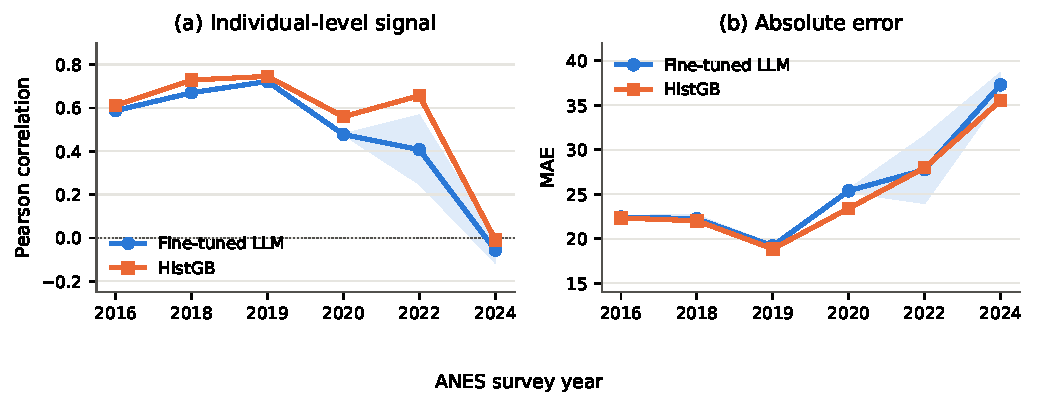
\includegraphics[width=\linewidth]{figures/fig2_temporal_decay.pdf}
\caption{Temporal decay of individual-level signal.}
\label{fig:temporal}
\end{figure*}

Two features of this pattern matter. First, the decay is not a sudden break at 2024; it begins between 2019 and 2020, the wave that includes the pandemic and the first Trump--Biden election. Second, the LLM decays earlier than the tabular baseline: by 2022 its correlation has fallen to 0.408 while HistGB is still at 0.657. A model that relies on a learned representation of partisan and ideological structure is apparently more sensitive to a changing political context than a model that relies on a small set of explicit features.

\subsection{The 2024 collapse}\label{the-2024-collapse}

On the full 2024 test set the collapse is complete. The fine-tuned LLM reaches an MAE of 36.47 \(\pm\) 0.75 but a correlation of -0.029 \(\pm\) 0.021; HistGB reaches 35.06 and -0.030. The predictions concentrate on the middle of the scale: 3,173 of 3,421 LLM predictions are exactly 50, and every Biden row is predicted as 50 (standard deviation 0.0), while Trump rows have a standard deviation of 17.4 and a correlation of -0.014. The anchor readout does not rescue the signal: on the same rows it produces a correlation of 0.003 with a prediction standard deviation of 2.1. The low ECE of the anchor readout (2.90) is therefore an artifact of near-constant predictions, not evidence of calibration.

This is not an LLM-specific failure. HistGB, which has no language-model component, also loses the individual signal in 2024. The common factor is the distribution shift in the survey itself: the 2024 wave is substantially more polarized, with a larger mass at the extremes and a smaller middle, than the waves used for training.

\subsection{Adding the most recent wave does not help}\label{adding-the-most-recent-wave-does-not-help}

A natural mitigation is to include the most recent available wave in training. We fine-tune the same model on the union of the 2016--2020 pool and the 2022 validation rows (9,017 rows) and evaluate on 2024. The result is essentially unchanged: MAE 36.62, correlation -0.030, choice 0.525, and a prediction standard deviation of 20.1. Adding 2022 does not restore the individual signal. This rules out a simple ``the model has not seen recent data'' explanation and points to a genuine distribution shift that one additional wave does not cover.

\subsection{Interpretation}\label{interpretation}

The temporal results support C3 in a strong form. Both the LLM and the tabular baseline learn a mapping that is valid for the 2016--2019 era but fails four years later. The LLM's earlier decay suggests that its representation is more tightly coupled to the training-era political structure; the tabular model's explicit features are more robust for one additional wave but fail in the same way at 2024. The practical implication is that a survey simulator trained on historical waves should not be used for a future election without a temporal validation protocol and, ideally, a domain-adaptation step. Reporting a single aggregate MAE over a pooled 2016--2024 test set would hide the collapse, because the pooled number is dominated by the earlier waves.

We therefore recommend that temporal shift be treated as a first-class evaluation axis for LLM survey simulation, alongside individual accuracy and distributional alignment. The negative result is informative: structured alignment is necessary but not sufficient for temporal generalization.

\subsection{Relation to the population-level results}\label{relation-to-the-population-level-results}

The FAS results in Section 6 are computed for a fixed target year with a reconstructed joint distribution, not for an unseen future wave. They therefore do not suffer from the same temporal shift, but they also do not demonstrate temporal extrapolation. The two components answer different questions: PAS asks whether the model can act as an individual respondent, FAS asks whether it can reproduce a population distribution. Neither, in our experiments, supports extrapolation to a substantially different political era.

\section{Ablations}\label{ablations}

\subsection{Setup}\label{setup-3}

We isolate three design choices with matched training runs. \textbf{A1 (random sampling)} replaces the nine-strategy pool with a uniform random sample of the same size (6,516 rows) from all cleaned 2016--2020 rows. \textbf{A2 (minimal prompt)} keeps the same rows but removes the interaction block from the prompt (party alignment, ideological distance, age difference). \textbf{A3 (name-only prompt)} additionally removes the candidate's party, position, and age, leaving only the candidate name. All three use the same LoRA configuration, three epochs, and seed 42; they are evaluated on the same in-distribution rows (2016--2019) as the main model. The full model is reported as the mean of seeds 42--44.

\subsection{Results}\label{results}

Table~\ref{tab:ablation} reports the results. The full model reaches an MAE of 20.84 \(\pm\) 0.24, a correlation of 0.679 \(\pm\) 0.003, and a choice accuracy of 0.553 \(\pm\) 0.011. A1 reaches 21.27, 0.658, and 0.543; A2 reaches 21.13, 0.670, and 0.567; A3 reaches 21.45, 0.657, and 0.565.

\begin{table}[t]
\centering
\small
\resizebox{\columnwidth}{!}{%
\begin{tabular}{lccc}
\toprule
Configuration & MAE & Correlation & Choice \\
\midrule
Full (9-strategy) & 20.84 $\pm$ 0.24 & 0.679 $\pm$ 0.003 & 0.553 $\pm$ 0.011 \\
A1 random sampling & 21.27 & 0.658 & 0.543 \\
A2 minimal prompt & 21.13 & 0.670 & 0.567 \\
A3 name-only prompt & 21.45 & 0.657 & 0.565 \\
\midrule
\multicolumn{4}{l}{\emph{Cross-pressure subgroups (MAE)}} \\
\midrule
Subgroup & LLM (3 seeds) & HistGB & $n$ \\
CP1 party vs.\ ideology & 18.77--21.55 & 21.55 & 154 \\
CP2 ideology vs.\ party & 23.21--24.13 & 23.18 & 318 \\
CP3 identity vs.\ party & 15.51--17.80 & 20.31 & 164 \\
No conflict & 20.45--21.09 & 20.14 & 2,090 \\
\bottomrule
\end{tabular}}
\caption{Ablations (top) and cross-pressure subgroups (bottom) on the 2016--2019 rows.}
\label{tab:ablation}
\end{table}



The direction is consistent: removing the distribution-aware sampling (A1) or the candidate metadata (A3) worsens MAE by roughly half a point and lowers the correlation by about 0.02. Removing the interaction block (A2) has a smaller effect on MAE and correlation, although it is still below the full model. Choice accuracy does not separate the conditions reliably; the differences are within the seed-level variation of the full model.

\subsection{Interpretation}\label{interpretation-1}

The ablations support a modest version of the data-design claim. The pipeline's sampling and metadata choices contribute a consistent 2--3\% improvement in MAE and a small gain in correlation, but they are not the main driver of the result. The interaction features, which are the most theoretically motivated part of the design, have the smallest measured effect in-distribution. This is worth stating plainly: the data-design story is real but small, and the paper should not claim that each component is individually necessary.

The small average effect does not mean the design is irrelevant. The sampling strategies target tails and cross-pressure cases that are rare in a uniform sample, and the cross-pressure analysis below shows where the model's behavior differs from the tabular baseline even when average MAE is similar.

\subsection{Cross-pressure subgroups}\label{cross-pressure-subgroups}

We classify each voter--candidate pair into three conflict types from Section 3.4 and compute MAE and correlation within each type on the 2016--2019 rows (Table~\ref{tab:ablation}, lower block). The fine-tuned LLM is substantially better than HistGB on CP3, the identity-versus-party conflict (MAE 15.51--17.80 across seeds versus 20.31 for HistGB), and comparable on CP1, the party-versus-ideology conflict (18.77--21.55 versus 21.55). It is slightly worse on CP2, the ideology-versus-party conflict (23.21--24.13 versus 23.18), and on the non-conflict rows (20.45--21.09 versus 20.14).

This is a finer-grained version of the main result: the LLM does not win on average, but it handles one theoretically important conflict type better than the feature-engineered baseline. The pattern is consistent across the three seeds, although each cell is small (154--318 rows), so we report it as a descriptive subgroup result rather than a confirmed advantage.

\subsection{Limitations}\label{limitations}

The ablations use one seed each, and the effects are small; a two- or three-seed replication would be needed to establish that the A1/A3 gaps are larger than run-to-run variation. The choice metric is noisier than MAE and should not be used to rank the ablations. Finally, the cross-pressure cells are small and the CP3 advantage should be treated as a hypothesis for future work rather than a settled finding.

\section{Limitations and Ethical Considerations}\label{limitations-and-ethical-considerations}

\textbf{Model coverage.} All fine-tuning experiments use Qwen3-8B. We were unable to evaluate a second model family: the Llama-3.1-8B weights are gated and the account used for this project was not authorized. We therefore cannot claim that the results are model-agnostic. The pipeline itself is model-agnostic---the training and readout code accepts any instruction-tuned causal LM---but the empirical claims are conditional on Qwen3-8B.

\textbf{Survey coverage.} The individual-level experiments use ANES and the population-level experiments use GSS, both from the United States. We do not test cross-national surveys, non-English questionnaires, or non-political attitude domains. The data-construction choices (candidate metadata, party and ideology features) are tailored to the ANES schema.

\textbf{Group attitudes.} We constructed a nine-group voter--group corpus and two evaluation protocols, but the group model was not evaluated in this paper. Group coverage is uneven across waves (three groups in 2016, nine in 2020, two in 2022), and the 2020 block lacks respondent identifiers. We therefore restrict the claims to candidate-level PAS and GSS FAS and leave the group analysis to future work.

\textbf{Panel structure.} ANES is a panel: 3,080 of 3,165 respondents appear in more than one wave, and there are no test-only respondents in 2022/2024. Our respondent protocol is disjoint by respondent, and our temporal protocol is disjoint by year, but the T\(\times\)R cell is small (226 rows). No protocol in this paper isolates a genuinely new respondent observed only in a future wave, because such respondents do not exist in the data.

\textbf{Choice metric.} Choice accuracy is rating-induced: we compare the model's highest-scoring candidate with the candidate with the highest ground-truth thermometer score, not with an observed vote. This avoids requiring a vote-choice variable for every wave, but it measures consistency with ratings rather than with behavior.

\textbf{Ablations.} The three ablations use one seed each. The effects are small (0.3--0.6 MAE), and a multi-seed replication would be needed to establish that they exceed run-to-run variation. The cross-pressure subgroup cells are also small (154--318 rows), and the CP3 advantage of the LLM should be treated as descriptive.

\textbf{Population-level results.} The FAS evaluation covers two three-attribute configurations. EDC improves strongly; EHC improves less, and the symmetric KL of the joint distribution moves in the opposite direction for direct SFT. The generated samples range from 351 to 400 valid rows, and we report both raw and coverage-adjusted metrics. The temporal extrapolation of the joint distribution is validated only for 2024; we do not test a longer horizon.

\textbf{Temporal mitigation.} We test one mitigation, adding the 2022 wave to training, and it does not help. We do not test domain adaptation, continual learning, uncertainty-aware decoding, or retrieval of recent survey statistics. The 2024 collapse is documented, not solved.

\textbf{Readout sensitivity.} Generation and anchor likelihood give different pictures. The anchor readout can produce a low ECE when predictions are nearly constant, and we therefore report correlation and prediction spread alongside ECE. The choice of readout should be treated as part of the method, not as a post-hoc detail.

\textbf{Ethical considerations.} Synthetic respondents are not a substitute for real survey participants. A model trained on historical data can reproduce and amplify the biases of that data, and its outputs can be mistaken for evidence about a population. The temporal results in this paper are a direct warning: a simulator that looks accurate in-distribution can lose all individual signal four years later. We recommend that any deployment report the training era, the validation protocol, the model family, and the coverage of the generated sample, and that synthetic results be clearly labeled as such. The ANES and GSS data are public and were used under their respective terms; no personally identifying information is released with this work.

\section{Conclusion}\label{conclusion}

We presented a data-centric pipeline for LLM survey simulation and evaluated it at three levels: the individual respondent, the population, and time. The pipeline reconstructs interaction-level data from ANES, decouples candidate identity from candidate attributes, encodes partisan and ideological structure as explicit features, samples the training pool to cover tails and conflict cases, and fine-tunes a compact 8B model with LoRA. The same pipeline reconstructs a joint distribution from GSS and fine-tunes a model to generate a synthetic population.

The individual-level result is deliberately modest. On unseen respondents in the same era, the fine-tuned model reaches an MAE of 20.84, a correlation of 0.679, and a choice accuracy of 0.518 against a chance level of 0.163. A gradient-boosted baseline on the same features reaches 20.58, 0.714, and 0.534. Paired bootstrap shows that the MAE and choice differences are not significant and that the baseline has a higher correlation. The value of the language model is not superior point prediction; it is a unified interface that produces a rating distribution and extends to population-level generation.

The population-level result is stronger, at least for the configuration with stable temporal trends. On EDC, fine-tuning reduces marginal and joint Jensen--Shannon divergence by 91\% and 86\% (93\% and 82\% for the fully covered run), and the gain is not explained by retrieval or quota sampling. On EHC the gain is real but smaller. The result supports the claim that structured alignment can make a compact model a usable population simulator, with the caveat that the claim is configuration-dependent.

The temporal result is the most important negative finding. Individual-level correlation falls from 0.722 in 2019 to -0.056 in 2024, and the tabular baseline collapses in the same way. Adding the most recent wave to training does not help. The failure is in the survey distribution, not in the language model alone. Structured alignment is necessary but not sufficient for temporal generalization, and temporal shift should be treated as a first-class evaluation axis.

Future work has four directions. First, replicate the pipeline on a second model family to test whether the individual-level tie with the tabular baseline is model-specific. Second, extend the evaluation to cross-national surveys and to the group-attitude corpus. Third, develop temporal adaptation methods---recency-weighted training, domain adaptation, or uncertainty-aware decoding---and evaluate them on the 2024 wave that defeats the current model. Fourth, study the choice metric against observed vote choice, so that rating-induced choice can be validated against behavior. We hope that the negative results reported here make the next round of work easier to calibrate.


\bibliographystyle{acl_natbib}
\bibliography{references}

\end{document}
